\documentclass{beamer}

\mode<presentation>
{
\useinnertheme{rounded}
\useoutertheme{infolines}
\usecolortheme{orchid}
\usecolortheme{whale}
}

\usepackage[english]{babel}
\usepackage[latin1]{inputenc}
\usepackage{times}
\usepackage[T1]{fontenc}
% Or whatever. Note that the encoding and the font should match. If T1
% does not look nice, try deleting the line with the fontenc.

\graphicspath{{../../modules/}}

\newtheoremstyle{partialproof}{3pt}{3pt}{}{}{}{.}{.5em}{}
\theoremstyle{partialproof} \newtheorem{partialproof}[theorem]{Proof.}
\DeclareMathOperator{\diff}{d}
\setbeamertemplate{navigation symbols}{}


\includeonlylecture{2}


% If you have a file called "university-logo-filename.xxx", where xxx
% is a graphic format that can be processed by latex or pdflatex,
% resp., then you can add a logo as follows:

%\pgfdeclareimage[height=0.8cm]{logo}{bluelogo}
%\logo{\pgfuseimage{logo}}

\begin{document}

\AtBeginLecture{%

\title[\insertlecture]{Math 140}
\subtitle{\insertlecture}
\author[Math 140]{Greg Maloney}
\institute[UMass Boston]{University of Massachusetts Boston}
\date{\insertshortlecture}
\begin{frame}
  \titlepage
\end{frame}

\begin{frame}{Outline}
  \tableofcontents[pausesections]
\end{frame}
}%

% begin lecture
\lecture[January 25, 2010]{Lecture 1}{1}
\section{(1.1) Four Ways to Represent a Function}
\subsection{Representations of Functions}
% begin module function-rep
\begin{frame}[t]
\frametitle{Representations of Functions}
There are four ways to represent a function:
\begin{enumerate}
\item<handout| 2-| alert@2>  Algebraically (by a formula).
\item<handout| 3-| alert@3>  Numerically (by a table of values).
\item<handout| 4-| alert@4>  Verbally (by a description in words).
\item<handout| 5-| alert@5>  Visually (by a graph).
\end{enumerate}

\only<handout:0| 2>{
\begin{example}[The Area of a Circle]
The area $A$ of a circle depends on its radius $r$.  The rule that connects $r$ and $A$ is given by the equation $A = \pi r^2$.  
\end{example}
}
\only<handout:0| 3>{
\begin{example}[The Human Population of the World]
\begin{columns}
\column{.7\textwidth}
The human population of the world $P$ depends on the time $t$.  The table on the right gives estimates of the world population $P(t)$ at time $t$, for certain years.  For example,
\[
P(2010) \approx 6,797,000,000 .
\]
\column{.3\textwidth}
\begin{tabular}{|c|c|}
\hline
 & Population \\
Year & (millions) \\
\hline
%1900 & 1650 \\
%1910 & 1750 \\
%1920 & 1860 \\
%1930 & 2070 \\
%1940 & 2300 \\
%1950 & 2560 \\
1960 & 3040 \\
1970 & 3710 \\
1980 & 4450 \\
1990 & 5280 \\
2000 & 6080 \\
2010 & 6797 \\
\hline
\end{tabular}
\end{columns}
\end{example}
}
\only<handout:0| 4>{
\begin{example}[The Cost of Mailing a Letter]
The cost $C$ of mailing a first-class letter depends on the weight $w$ of the letter.  Although there is no simple formula that connects $w$ and $C$, the post office has a rule for determining $C$ when $w$ is known.
\end{example}
}
\only<handout:0| 5>{
\begin{example}[ECG Readings]
The electrical activity of the heart, as recorded by an electrocardiograph machine, is a function of the elapsed time $t$.  The graph below depicts the ECG data recorded for a patient at a hospital.

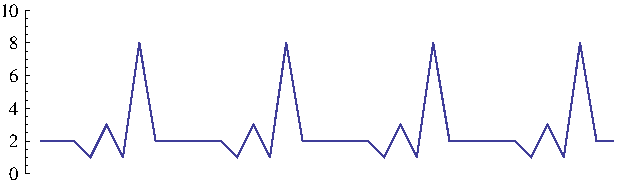
\includegraphics[height=2.5cm]{precalculus/pictures/01-01-ECG.pdf}

\end{example}
}
\end{frame}


\begin{frame}
\frametitle{The Definition of a Function}

\begin{definition}[Function]
A function $f$ is a rule that assigns to each element $x$ in a set $D$ exactly one element, called $f(x)$, in a set $E$.
\end{definition}

\uncover<2->{
\begin{definition}[Domain and Range]
The set $D$ is called the domain and $E$ is called the range.  We consider functions for which the domain and range are sets of real numbers.
\end{definition}
}

\uncover<3->{
\begin{definition}[Value of $f$ at $x$]
The number $f(x)$ is called the value of $f$ at $x$, and is read ``$f$ of $x$.''
\end{definition}
}

\uncover<4->{
\begin{definition}[Independent and Dependent Variables]
A symbol that represents an arbitrary number in the domain is called an independent variable.  A symbol that represents an arbitrary number in the range is called a dependent variable.
\end{definition}
}
\end{frame}
% end module function-rep

% begin module function-def
\begin{frame}
\psset{xunit=1.1cm,yunit=1.1cm}
\begin{pspicture}(-1,-1)(4,3)
\tiny
\psaxes[labels=none, ticks=none]{->}(0,0)(-0.5,-0.5)(4,3)
\rput[r](0,3){$y$}
\rput[l](4,0){$x$}
\psplot[linecolor=red]{0.5}{3}{0.2 x 2 exp mul 0.5 180 x mul sin mul 0.333333 add add
 }
\rput( 3, 2.5){$y=f(x)$}

\only<3>{
\psline[linecolor=red, linewidth=2pt]{<->}(0.5, 0)(3,0)
\rput(1.75, -0.3){\color{red}Domain}
}
\only<4>{
\psline[linecolor=blue, linewidth=2pt]{<->}(0, -0.5)(0,3)
\rput[l](0.05, 2.35){\color{blue}Co-Domain}
}
\only<5>{
\psline[linewidth=1pt](2.166666667, 0)(2.166666667, 1.522222)
\rput[l](2.2,0.7){$f(x)$}
\rput[t](2.2, -0.1){$x$}
}
\only<8>{
\psline[linecolor=purple, linewidth=3pt]{<->}(0, 0.245)(0,2.205)
\rput[l](0.05, 1.1){\color{purple}Range}
\psline[linestyle=dashed](0,0.245)(1.4, 0.245)
\psline[linestyle=dashed](0,2.205)(2.75, 2.205)
}
\end{pspicture}
\begin{definition}[Function]
A function $f$ is a rule that assigns to each element $x$ in a set $D$ exactly one element, called $f(x)$, in a set $E$.
\end{definition}

\only<handout:1| 2-3>{
\begin{itemize}
\item Functions are also synonymously called ``maps''.
\end{itemize}

\uncover<3->{
\begin{definition}[Domain]
The set $D$ in the definition of $f$ is called the domain of $f$. 
\end{definition}
}
}

\only<handout:2| 4>{
\begin{definition}[Co-domain]
The set $E$ in the definition of $f$  is called the co-domain of $f$. 
\end{definition}
}

\only<handout:3| 5-7>{
\begin{definition}[Value of $f$ at $x$]
The number $f(x)$ is called \emph{the value of $f$ at $x$} and is read ``$f$ of $x$''.
\end{definition}

\begin{itemize}
\item<6-> The value of $f$ at $x$ is also called the image of $x$ under the map $f$.
\item<7-> In the expression $f(x)$, $x$ is referred to as the \emph{argument} of $f$. 
\end{itemize}
}
\only<handout:4| 8->{
\begin{definition}[Range]
The set of all possible values taken by $f(x)$ as the element $x$ runs over elements of $D$ is called the range of $f$. 
\end{definition}
}

\vskip 10cm 


\end{frame}
% end module function-def
% begin module function-machine
\begin{frame}
It is often helpful to view a function as a machine.  If $x$ is an element of $D$, then the machine takes $x$ as input and produces $f(x)$, an element of $E$, as output.

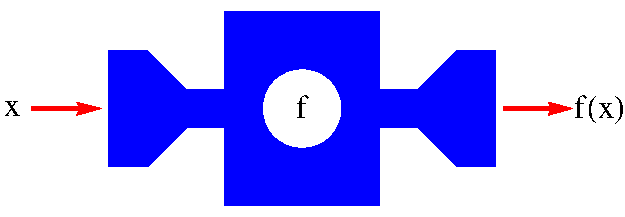
\includegraphics[height=4cm]{precalculus/pictures/01-01-machine.pdf}
\end{frame}
% end module function-machine

\subsection{Piecewise Defined Functions}
% begin module function-piecewise
\begin{frame}
\frametitle{Piecewise Defined Functions}
\begin{definition}[Piecewise Defined Function]
A piecewise defined function is a function that is defined by different algebraic formulas on different subsets of its domain.
\end{definition}
\uncover<2->{
\begin{example}
\begin{columns}[t]
\column{.4\textwidth}
\psset{xunit=0.8cm, yunit=0.8cm}
\begin{pspicture}(-5, -5)(5,5) 
\psframe*[linecolor=white](-5,-5)(5,5) 
\psaxes[ticks=none, labels=none]{<->}(0,0)(-3,-1.5)(3,1.5)\tiny
\psLabelsWithOnes{3}{1.5}
\psline[linecolor=red](-3, -1)(0,-1)
\psline[linecolor=red](3, 1)(0,1)
\psHollowDot{0}{-1}
\psFullDot{0}{1}
\end{pspicture} 
%\ 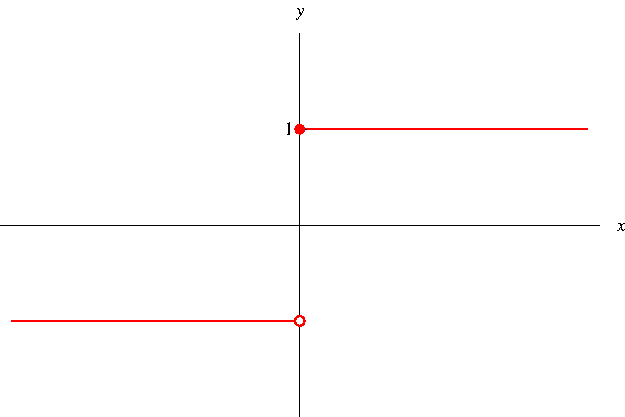
\includegraphics[height=3.5cm]{precalculus/pictures/01-01-piecewise.pdf}
\column{.5\textwidth}
\[
f(x) = \left\{ \begin{array}{rcc}
1 & \textrm{ if } & x \geq 0 \\
-1 & \textrm{ if } & x < 0 
\end{array}\right. 
\]

The filled red circle means $(0,1)$ is on the curve.  

The open circle means $(0, -1)$ is not on the curve.
\end{columns}
\end{example}
}
\end{frame}
% end module function-piecewise

% begin module absolute-value
\begin{frame}
\begin{example}
The absolute value $|x|$ of a number $a$ is defined to be
\[
|x| = \left\{ \begin{array}{ccccl}
\alertNoH{ 2-3}{x} & \alertNoH{ 3}{\text{if}} & \alertNoH{ 3}{x} & \alertNoH{ 3}{\geq} & \alertNoH{ 3}{0} \\
\alertNoH{ 4-5}{-x} & \alertNoH{ 5}{\text{if}} &  \alertNoH{ 5}{x} & \alertNoH{ 5}{<} & \alertNoH{ 5}{0}. \end{array}\right.
\]

Sketch a graph of the function $f(x) = |x|$.

%no begin{center} due to bug!
\hfil\hfil
\psset{xunit=1.2cm, yunit=1.2cm}
\begin{pspicture}(-3.2, -0.5)(3.2,3.2)
\tiny
\psframe*[linecolor=white](-3.2,-0.5)(3.2,3.2)
\psaxes[ticks=none, labels=none]{<->}(0,0)(-3,-0.5)(3,3)
\fcLabelsWithOnes{3}{3}
\uncover<handout:0|2>{
\psline[linecolor=blue](-0.5, -0.5)(3,3)
}
\uncover<3->{
\psline[linecolor=red](0,0)(3,3)
}
\uncover<handout:0|4>{
\psline[linecolor=blue](-3, 3)(0.5,-0.5)
}
\uncover<5->{
\psline[linecolor=red](-3, 3)(0,0)
}
\end{pspicture}
\end{example}
\end{frame}
% end module absolute-value

% begin module piecewise-formula
\begin{frame}
\begin{example} %[Example 9, p. 18]
Find a formula for the function $f$ in the graph.

\psset{xunit=1.2cm, yunit=1.2cm}
\begin{pspicture}(-0.5, -0.5)(5.3,2.4)
\tiny
\psframe*[linecolor=white](-0.5,-0.5)(5.2,2.4)
\psaxes{<->}(0,0)(-0.5,-0.5)(5.2,2.2)
\fcLabels{5.1}{2.2}
\psline[linecolor=red](0,0)(1,1)(2,0)(5,0)
\fcHollowDot{5}{0}
\fcFullDot{0}{0}
\only<handout:0|4-5>{
\psline[linecolor=blue](-0.5, -0.5)(2,2)
}
\only<handout:0|6-7>{
\psline[linecolor=blue](-0.2, 2.2)(2.5,-0.5)
}
\only<handout:0|8-9>{
\psline[linecolor=blue](2, 0)(5,0)
}
\end{pspicture}
%\ \only<1-3,10>{%
%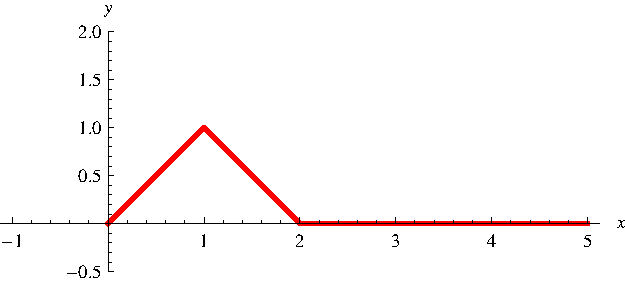
\includegraphics[height=4cm]{precalculus/pictures/01-01-ex-09a.pdf}%
%}%
%\only<handout:0| 4-5>{%
%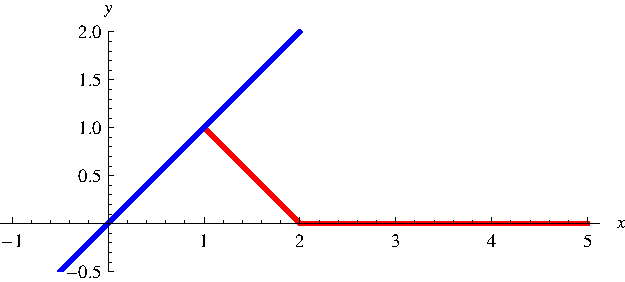
\includegraphics[height=4cm]{precalculus/pictures/01-01-ex-09b.pdf}%
%}%
%\only<handout:0| 6-7>{%
%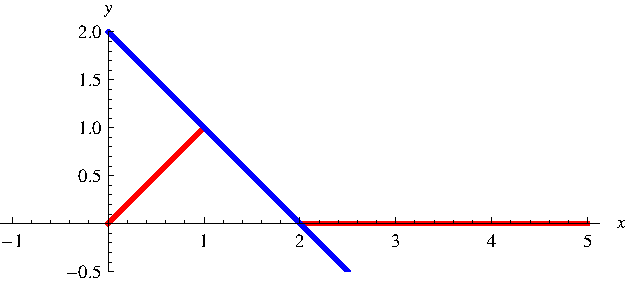
\includegraphics[height=4cm]{precalculus/pictures/01-01-ex-09c.pdf}%
%}%
%\only<handout:0| 8-9>{%
%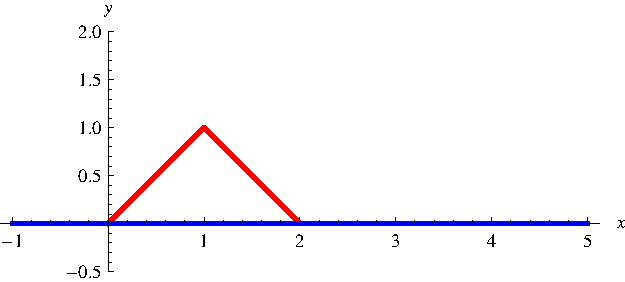
\includegraphics[height=4cm]{precalculus/pictures/01-01-ex-09d.pdf}%
%}%

\uncover<2->{
Different formulas on $[0, 1)$, $[1, 2)$, and $[2, 5)$.
}

\uncover<3->{
\[
f(x) = \left\{ \begin{array}{ccccccl}
\uncover<5->{\alert<handout:0| 5>{x}} & \alert<handout:0| 4-5>{\textrm{if}} & \alert<handout:0| 4-5>{0} & \alert<handout:0| 4-5>{\leq} & \alert<handout:0| 4-5>{x} & \alert<handout:0| 4-5>{<} & \alert<handout:0| 4-5>{1} \\
\uncover<7->{\alert<handout:0| 7>{2 - x}} & \alert<handout:0| 6-7>{\textrm{if}} & \alert<handout:0| 6-7>{1} & \alert<handout:0| 6-7>{\leq} & \alert<handout:0| 6-7>{x} & \alert<handout:0| 6-7>{<} & \alert<handout:0| 6-7>{2} \\
\uncover<9->{\alert<handout:0| 9>{0}} & \alert<handout:0| 8-9>{\textrm{if}} & \alert<handout:0| 8-9>{2} & \alert<handout:0| 8-9>{\leq} & \alert<handout:0| 8-9>{x} & \alert<handout:0| 8-9>{<} & \alert<handout:0| 8-9>{5} \end{array}\right.
\]
}
\end{example}
\end{frame}
% end module piecewise-formula

\subsection{Symmetry}
% begin module even-and-odd
\begin{frame}
\frametitle{Symmetry}
\begin{definition}[Even and Odd Functions]
A function $f$ is called even if $f(-x) = f(x)$ for all $x$ in its domain.  A function $f$ is called odd if $f(-x) = -f(x)$ for all $x$ in its domain.
\end{definition}
\uncover<2->{
\begin{example}[$x^2$ is Even, $x^3$ is Odd]
The function $f(x) = x^2$ is even:
\uncover<3->{
\[
f(-x) = (-x)^2 = x^2 = f(x) .
\]
}
The function $g(x) = x^3$ is odd:
\uncover<4->{
\[
g(-x) = (-x)^3 = -x^3 = -g(x) .
\]
}
\end{example}
}
\end{frame}

\begin{frame}
\begin{definition}[Even and Odd Functions]
A function $f$ is called even if $f(-x) = f(x)$ for all $x$ in its domain.  A function $f$ is called odd if $f(-x) = -f(x)$ for all $x$ in its domain.
\end{definition}
\begin{example} %[Example 11, p. 19]
Determine whether each of the following functions is even, odd, or neither even nor odd.

\begin{columns}[t]
\column{.33\textwidth}
\[
f(x) = x^5 + x
\]
\[
\begin{array}{r@{ \ }c@{ \ }l}
\uncover<2->{f(-x)} & \uncover<2->{=} & \uncover<3->{(-x)^5 + (-x)} \\
& \uncover<4->{=} & \uncover<4->{-x^5 - x} \\
& \uncover<5->{=} & \uncover<5->{-(x^5 + x)} \\
& \uncover<6->{=} & \uncover<6->{-f(x)} 
\end{array}
\]
\uncover<7->{
Therefore $f$ is odd.
}
\column{.33\textwidth}
\[
g(x) = 1 - x^4
\]
\[
\begin{array}{r@{ \ }c@{ \ }l}
\uncover<2->{g(-x)} & \uncover<2->{=} & \uncover<8->{1 - (-x)^4} \\
& \uncover<9->{=} & \uncover<9->{1 - x^4} \\
& \uncover<10->{=} & \uncover<10->{g(x)} 
\end{array}
\]
\uncover<11->{
Therefore $g$ is even.
}
\column{.33\textwidth}
\[
h(x) = 2x - 1
\]
\[
\begin{array}{r@{ \ }c@{ \ }l}
\uncover<2->{h(-x)} & \uncover<2->{=} & \uncover<12->{2(-x) - 1} \\
& \uncover<13->{=} & \uncover<13->{-2x - 1} \\
& \uncover<14->{\neq} & \uncover<14->{h(x), -h(x)}
\end{array}
\]
\uncover<15->{
Therefore $h$ is neither even nor odd.
}
\end{columns}
\end{example}
\end{frame}
% end module even-and-odd

\subsection{Increasing and Decreasing Functions}
% begin module increasing-decreasing
\begin{frame}
\frametitle{Increasing and Decreasing Functions}
\begin{definition}[Increasing and Decreasing Functions]
A function $f$ is called increasing on an interval $I$ if $f(x_1) < f(x_2)$ whenever $x_1 < x_2$  in $I$.

It is called decreasing on the interval $I$ if $f(x_1) > f(x_2)$ whenever $x_1 < x_2$ in $I$.
\end{definition}
\uncover<2->{
\begin{example}[Increasing and Decreasing]
\begin{columns}[t]
\column{.6\textwidth}

\psset{xunit=3.4cm, yunit=3.4cm}
\begin{pspicture}(-1.1, -0.4)(1.15,0.7)
\psframe*[linecolor=white](-1.1,-0.4)(1.15,0.7)
\tiny
\psaxes[Dx=0.25, Dy=0.25]{<->}(0,0)(-1.1,-0.3)(1.1,0.6)
\fcLabels{1.1}{0.6}
%Function formula: 7/40+13/10 ((x)^{3})-39/40 (x)
\psplot[linecolor=red, plotpoints=1000]{-1}{1}{x -0.975 mul x 3 exp 1.3 mul 0.175 add add }
\uncover<handout:0|3>{
\psplot[linecolor=blue, plotpoints=1000]{-1}{-0.5}{x -0.975 mul x 3 exp 1.3 mul 0.175 add add }
}
\uncover<handout:0|4>{
\psplot[linecolor=blue, plotpoints=1000]{-0.5}{0.5}{x -0.975 mul x 3 exp 1.3 mul 0.175 add add }
}
\uncover<handout:0|5>{
\psplot[linecolor=blue, plotpoints=1000]{0.5}{1}{x -0.975 mul x 3 exp 1.3 mul 0.175 add add }
}
\end{pspicture}
%\ \only<-2>{%
%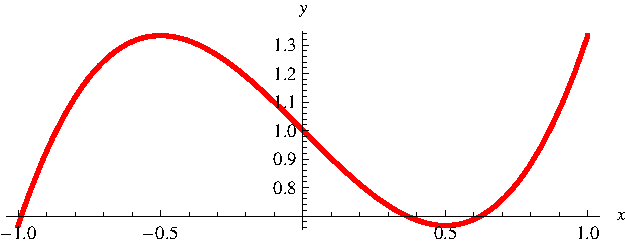
\includegraphics[height=2.8cm]{precalculus/pictures/01-01-inc-dec-a.pdf}%
%}%
%\only<handout:0| 3>{%
%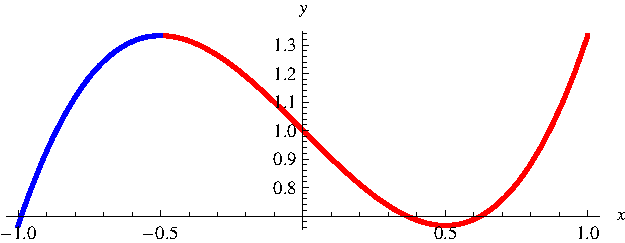
\includegraphics[height=2.8cm]{precalculus/pictures/01-01-inc-dec-b.pdf}%
%}%
%\only<handout:0| 4>{%
%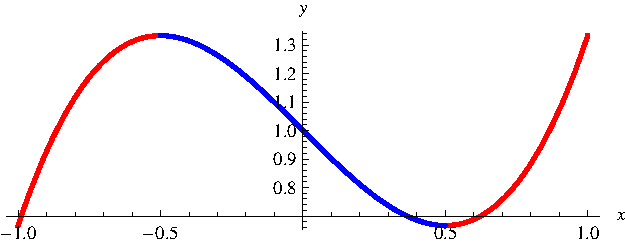
\includegraphics[height=2.8cm]{precalculus/pictures/01-01-inc-dec-c.pdf}%
%}%
%\only<handout:0| 5->{%
%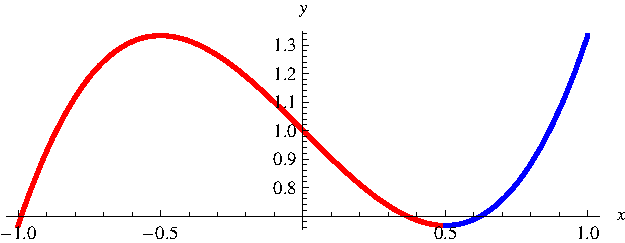
\includegraphics[height=2.8cm]{precalculus/pictures/01-01-inc-dec-d.pdf}%
%}%
\column{.4\textwidth}
\begin{itemize}
\item<3-| alert@3> \only<handout:0|3>{\color{blue}} $f$ is increasing on $[-1, -\frac{1}{2}]$.
\item<4-| alert@4> \only<handout:0|4>{\color{blue}} $f$ is decreasing on $[-\frac{1}{2}, \frac{1}{2}]$.
\item<5-| alert@5> \only<handout:0|5>{\color{blue}} $f$ is increasing on $[\frac{1}{2}, 1]$.
\end{itemize}
\end{columns}
\end{example}
}
\end{frame}
% end module increasing-decreasing

% end lecture

% begin lecture
\lecture[January 27, 2010]{Lecture 2}{2}
\section{(1.1) Four Ways to Represent a Function}
\subsection{The Vertical Line Test}
% begin module vertical-line-test
\begin{frame}
\frametitle{The Vertical Line Test}
\begin{question}
Given a curve in the plane, is it the graph of a function or not?
\end{question}

\uncover<2->{The answer is as follows.
\begin{proposition}[The Vertical Line Test]
A curve in the plane is the graph of a function if and only if no vertical line intersects it more than once.
\end{proposition}
}

\begin{tabular}{ccc}
\psset{xunit=0.33cm, yunit=0.33cm}
\begin{pspicture}(-5, -5)(5,5) 
\psframe*[linecolor=white](-5,-5)(5,5) 
\psaxes[ticks=none, labels=none]{<->}(0,0)(-4.5,-4.5)(4.5,4.5)\tiny
%Function formula: sin{}(x) 
\psplot[linecolor=red, plotpoints=1000]{-5}{5}{x 57.29578 mul sin }
\end{pspicture}
%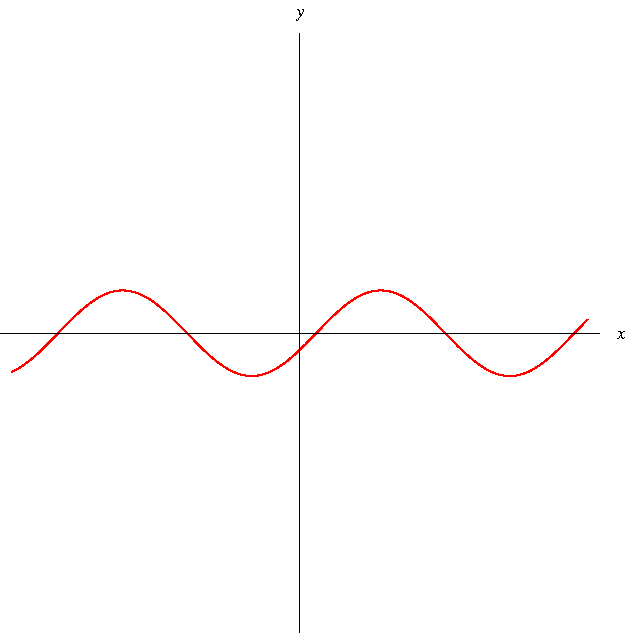
\includegraphics[height=3.8cm]{precalculus/pictures/01-02-vlt3.pdf} 
&%
\psset{xunit=0.33cm, yunit=0.33cm}
\begin{pspicture}(-5, -5)(5,5) 
\psframe*[linecolor=white](-5,-5)(5,5) 
\psaxes[ticks=none, labels=none]{<->}(0,0)(-4.5,-4.5)(4.5,4.5)\parametricplot[linecolor=red, plotpoints=1000]{0.05}{3}{t t 2.2 mul 57.29578 mul sin 1 add add t 57.29578 mul cos mul t t 2.2 mul 57.29578 mul sin 1 add add t 57.29578 mul sin mul}
\only<handout| 6->{%
\psline(1.7, -4.5)(1.7, 4.5)
}
\end{pspicture}
%\only<handout:0| -2>{%
%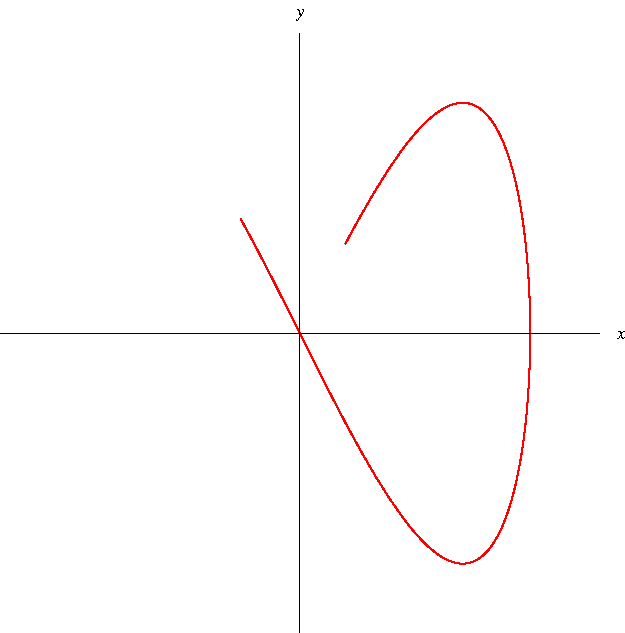
\includegraphics[height=3.8cm]{precalculus/pictures/01-02-vlt1a.pdf}%
%}%
%\only<handout| 3->{%
%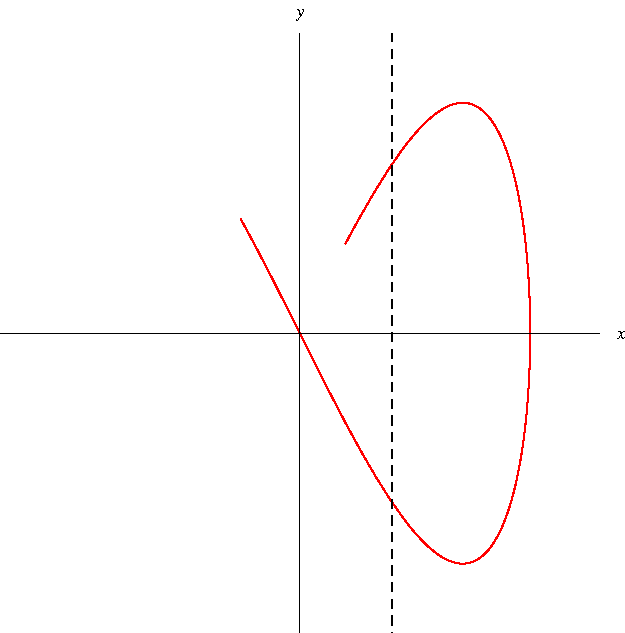
\includegraphics[height=3.8cm]{precalculus/pictures/01-02-vlt1b.pdf}%
%} 
&%
\psset{xunit=0.33cm, yunit=0.33cm}
\begin{pspicture}(-5, -5)(5,5) 
\psframe*[linecolor=white](-5,-5)(5,5) 
\psaxes[ticks=none, labels=none]{<->}(0,0)(-4.5,-4.5)(4.5,4.5)\tiny
%Function formula: 3/8+3/2 ((x)^{2})+1/4 (x)- ((x)^{3}) 
\psplot[linecolor=red, plotpoints=1000]{-0.5}{2}{x 3 exp -1 mul x 0.25 mul x 2 exp 1.5 mul 0.375 add add add } %Function formula: 1+1/2 (x) 
\psplot[linecolor=red, plotpoints=1000]{-4}{-0.5}{x 0.5 mul 1 add }
\end{pspicture} 
%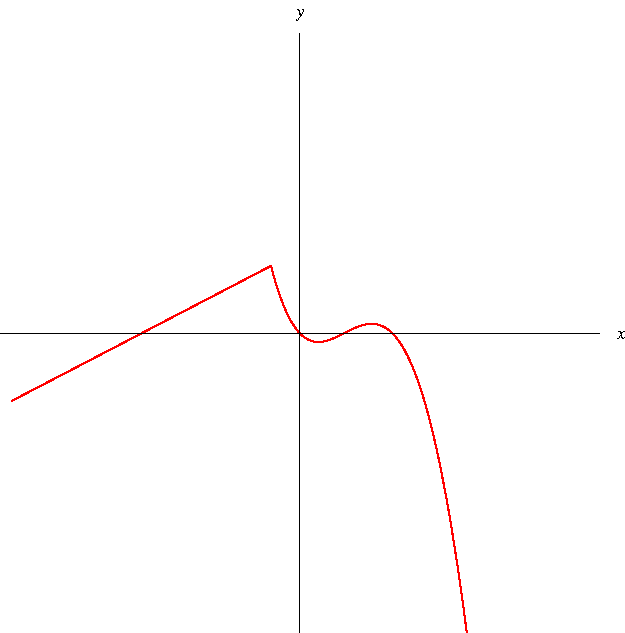
\includegraphics[height=3.8cm]{precalculus/pictures/01-02-vlt2.pdf} 
\\%
\fcAnswerUncoverNoH{1}{4}{Function} &
\fcAnswerUncoverNoH{1}{6}{Not a function}&
\fcAnswerUncoverNoH{1}{8}{Function}
\end{tabular}
\end{frame}
% end module vertical-line-test

\section{(1.2) A Catalog of Essential Functions}
\subsection{Linear Functions}
% begin module linear-functions
\begin{frame}
\frametitle{Linear Functions}
\begin{definition}[Linear Function]
A linear function is a function the graph of which is a line.  We can write any linear function in slope-intercept form:
\[
f(x) = mx + b.
\]
$m$ is called the slope, and $b$ is called the $y$-intercept.
\end{definition}
\end{frame}

\begin{frame}
\begin{columns}[c]
\column{.5\textwidth}

\psset{xunit=0.7cm, yunit=0.7cm}
\begin{pspicture}(-2.6, -2.5)(5,2.6)
\psframe*[linecolor=white](-2.6,-2.5)(4.1,2.6)
\tiny
\fcAxesStandard{-2.6}{-2.5}{5}{2.6}
\fcLabelXOne
\uncover<2>{
\psline[linecolor=red](-2.5, -1.5)(1.5, 2.5)
}
\uncover<3->{
\psline[linecolor=blue](-2.5, -1.5)(1.5, 2.5)
}
\uncover<2->{
\rput[l](1.5, 2){$y=x+1$}
}
\uncover<5->{
\fcFullDot{0}{1}
\rput[r](-0.1, 1){\alert<5>{$(0,1)$}}
}

\uncover<3>{
\psline[linecolor=red](-2.5, 1.25)(5, -2.5)
}
\uncover<4->{
\psline[linecolor=blue](-2.5, 1.25)(5, -2.5)
}
\uncover<3->{
\rput[r](3.3, -2){$y=-0.5x$}
}
\uncover<6->{
\fcFullDot{0}{0}
\rput[lb](0.1, 0.1){\alert<6>{$(0,0)$}}
}

\uncover<4>{
\psline[linecolor=red](-2.5,-1)(5, -1)
}
\uncover<5->{
\psline[linecolor=blue](-2.5, -1)(5, -1)
}
\uncover<4->{
\rput[t](4, -1.1){$y=-1$}
}
\uncover<7->{
\fcFullDot{0}{-1}
\rput[lt](0.1, -1.1){\alert<7>{$(0,-1)$}}
}
\end{pspicture}
\column[t]{.55\textwidth}
\begin{tabular}{|c|c|c|}
\hline
$f(x)$ & Direction & $y$-intercept \\
\hline
\uncover<1->{\alert<handout:0| 2>{$x + \alert<handout:0| 5>{1}$}} &
\uncover<2->{\alert<handout:0| 2>{$\nearrow$}} &
\uncover<5->{\alert<handout:0| 5>{1}} \\
\uncover<1->{\alert<handout:0| 3>{$-0.5x \uncover<6>{\alert<handout:0| 6>{+ 0}}$}} &
\uncover<3->{\alert<handout:0| 3>{$\searrow$}} &
\uncover<6->{\alert<handout:0| 6>{0}} \\
\uncover<1->{\alert<handout:0| 4,7>{$-1$}} &
\uncover<4->{\alert<handout:0| 4>{$\rightarrow$}} &
\uncover<7->{\alert<handout:0| 7>{-1}} \\
\hline
\end{tabular}
\end{columns}

\begin{itemize}
\item<2->  $m > 0$ means the graph of $f$ points up ($\nearrow$).
\item<3->  $m < 0$ means the graph of $f$ points down ($\searrow$).
\item<4->  $m = 0$ means the graph of $f$ is horizontal ($\rightarrow$).
\item<5->  $b$ tells us the height of the point where the graph hits the $y$-axis.
\end{itemize}
\end{frame}
% end module linear-functions

\subsection{Polynomials}
% begin module polynomials
\begin{frame}
\frametitle{Polynomials}
\begin{definition}[Polynomial Function]
A polynomial function is a function $f$ of the form
\[
f(x) = a_0 + a_1x + a_2x^2 + \cdots + a_{n - 1}x^{n-1} + a_nx^n ,
\]
where $n$ is a non-negative integer and $a_0, \ldots , a_n$ are real numbers, called the coefficients.

If the leading coefficient $a_n \neq 0$, then we say the degree of $f$ is $n$.
\end{definition}
\uncover<2->{
\[
\begin{array}{|c|c|c|c|c|c|}
\hline
f(x) &%
\alert<handout:0| 3-4,13-14,23-26,35-36>{\text{Polynomial?}} &%
\alert<handout:0| 5-6,15-16,27-28>{\text{Degree}} &%
\alert<handout:0| 7-8,17-18,29-30>{a_0} &%
\alert<handout:0| 9-10,19-20,31,32>{a_1} &%
\alert<handout:0| 11-12,21-22,33-34>{a_2} \\
\hline
\alert<handout:0| 3-12>{x^4-x+1} &%
\uncover<4->{\alert<handout:0| 4>{\text{Yes}}}&%
\uncover<6->{\alert<handout:0| 6>{4}}&%
\uncover<8->{\alert<handout:0| 8>{1}}&%
\uncover<10->{\alert<handout:0| 10>{-1}}&%
\uncover<12->{\alert<handout:0| 12>{0}}\\%
\alert<handout:0| 13-22>{6} &%
\uncover<14->{\alert<handout:0| 14>{\text{Yes}}}&%
\uncover<16->{\alert<handout:0| 16>{0}}&%
\uncover<18->{\alert<handout:0| 18>{6}}&%
\uncover<20->{\alert<handout:0| 20>{0}}&%
\uncover<22->{\alert<handout:0| 22>{0}}\\%
\alert<handout:0| 23>{3x^2 - \frac{1}{2}x + \alert<handout:0| 24>{\sqrt{x}}} &%
\uncover<24->{\alert<handout:0| 24>{\text{No}}}&%
&%
&%
&\\
\alert<handout:0| 25-34>{3x^2 - \frac{1}{2}x + \sqrt{2}} &%
\uncover<26->{\alert<handout:0| 26>{\text{Yes}}}&%
\uncover<28->{\alert<handout:0| 28>{2}}&%
\uncover<30->{\alert<handout:0| 30>{\sqrt{2}}}&%
\uncover<32->{\alert<handout:0| 32>{-\frac{1}{2}}}&%
\uncover<34->{\alert<handout:0| 34>{3}}\\%
\alert<handout:0| 35>{3x^2 - \frac{1}{2\alert<handout:0| 36>{x}} + \sqrt{2}} &%
\uncover<36->{\alert<handout:0| 36>{\text{No}}}&%
&%
&%
&\\
\hline
\end{array}
\]
}
\end{frame}


\begin{frame}
\begin{itemize}
\item<1->  Linear functions are polynomials.
\item<2->  So are quadratic functions.  Their graphs are parabolas.
\item<3->  And there are many more.
\end{itemize}
\only<handout:1| 1>{%
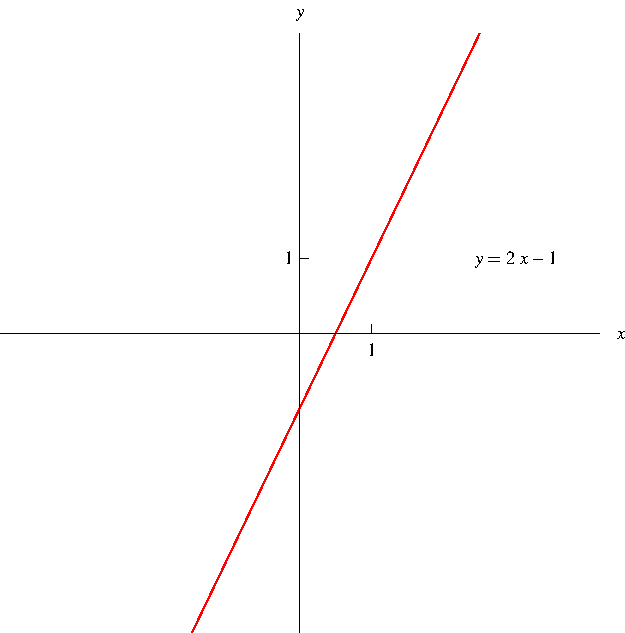
\includegraphics[height=6cm]{precalculus/pictures/01-02-line.pdf}%

Linear
}%
\only<handout:2| 2>{%
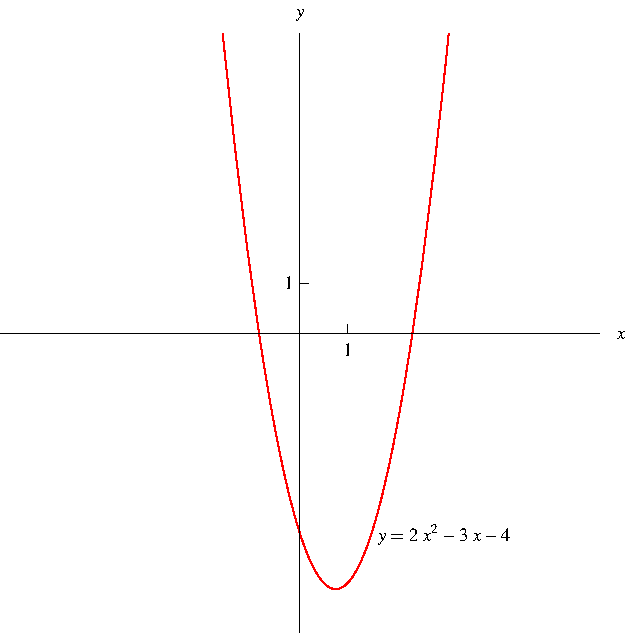
\includegraphics[height=6cm]{precalculus/pictures/01-02-parabola.pdf}%

Quadratic
}%
\only<handout:3| 3>{%
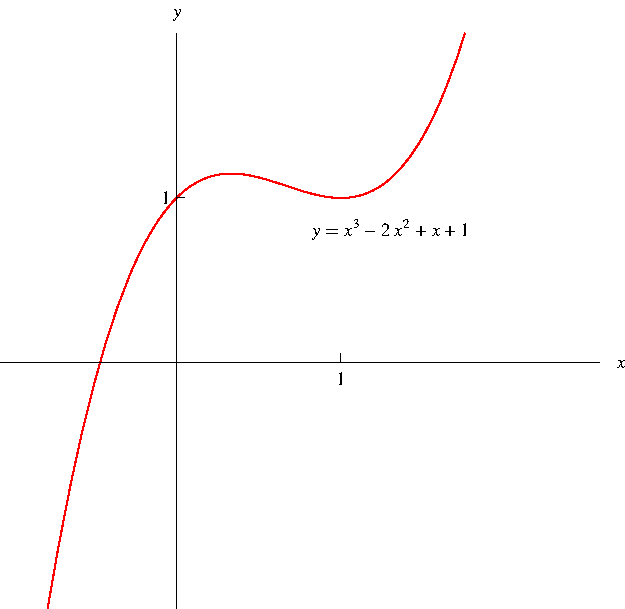
\includegraphics[height=6cm]{precalculus/pictures/01-02-polya.pdf}%

Cubic
}%
\only<handout:4| 4>{%
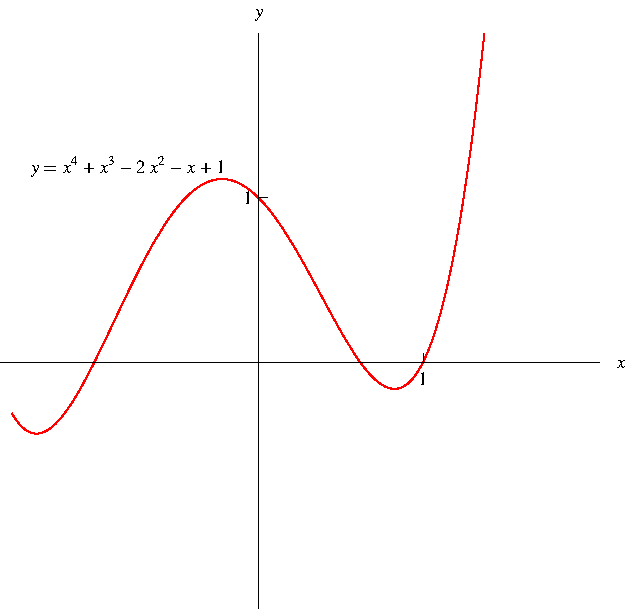
\includegraphics[height=6cm]{precalculus/pictures/01-02-polyb.pdf}%

Quartic
}%
\only<handout:5| 5>{%
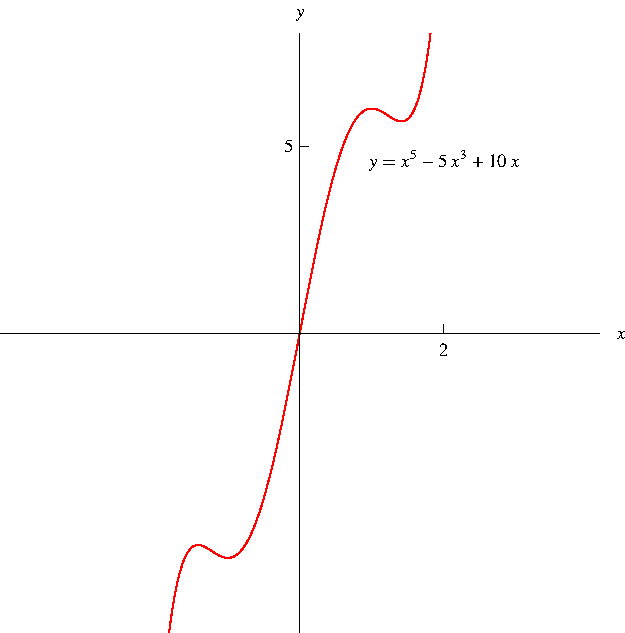
\includegraphics[height=6cm]{precalculus/pictures/01-02-polyc.pdf}%

Quintic
}
\end{frame}
% end module polynomials

\subsection{Power Functions}
%Old Version from Greg. Greg, this slide is changed substantially, please take a look.
%% begin module power-functions-def
%\begin{frame}
%\frametitle{Power Functions}
%\begin{definition}[Power Function]
%A power function is a function of the form
%\[
%f(x) = x^a,
%\]
%where $a$ is a fixed real number.
%\end{definition}
%\uncover<2->{
%If $a$ is a positive integer like $1, 2, 3, \ldots$ then $x^a$ is a polynomial.

%\only<handout:-2| -2>{%
%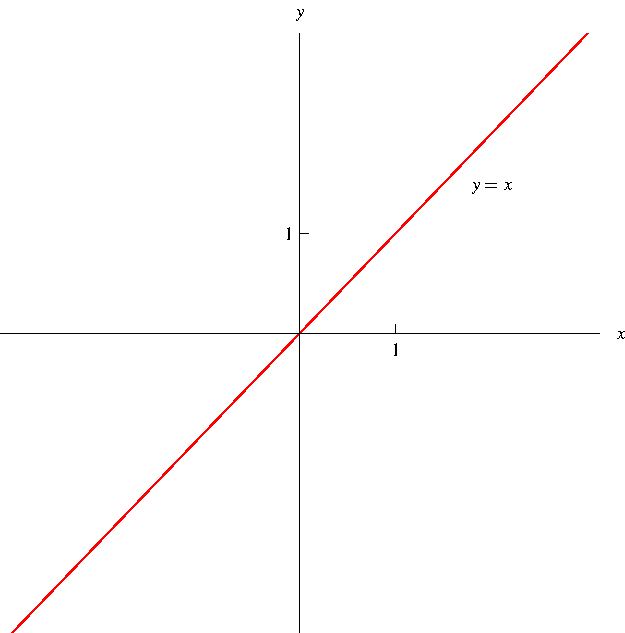
\includegraphics[height=4cm]{precalculus/pictures/01-02-x.pdf}%
%}%
%\only<handout:3| 3>{%
%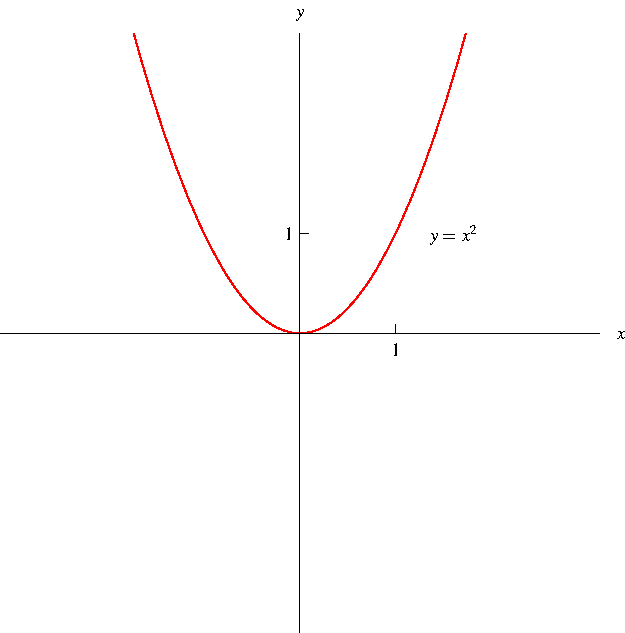
\includegraphics[height=4cm]{precalculus/pictures/01-02-xsquared.pdf}%
%}%
%\only<handout:4| 4>{%
%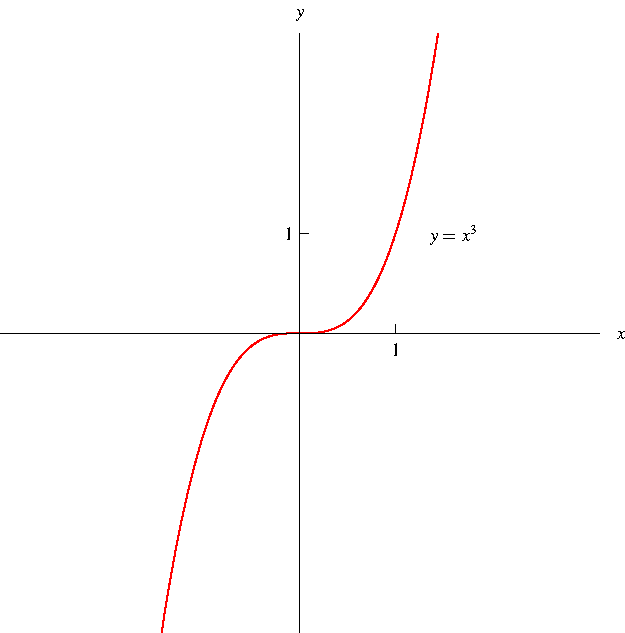
\includegraphics[height=4cm]{precalculus/pictures/01-02-xcubed.pdf}%
%}%
%\only<handout:5| 5>{%
%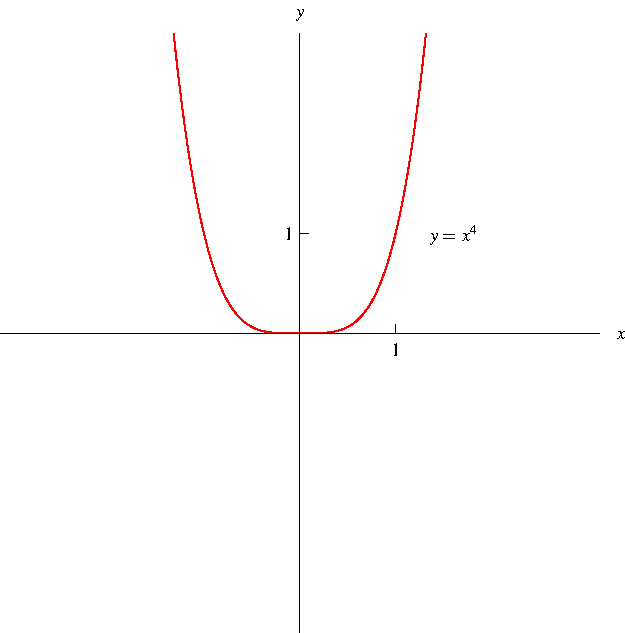
\includegraphics[height=4cm]{precalculus/pictures/01-02-xfourth.pdf}%
%}%
%\only<handout:6| 6>{%
%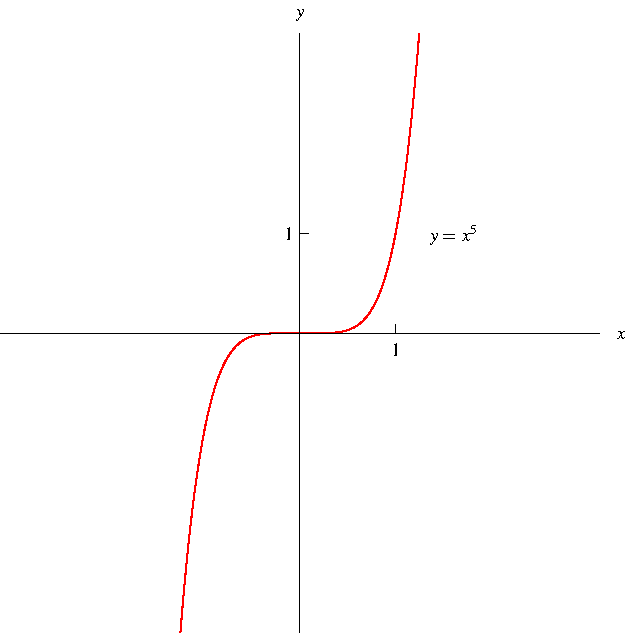
\includegraphics[height=4cm]{precalculus/pictures/01-02-xfifth.pdf}
%}%
%}%
%\end{frame}
%% end module power-functions-def

% begin module power-functions-def
\begin{frame}[t]
\frametitle{Power Functions}
\begin{definition}[Power Function]
Let $x>0$, $a$ - arbitrary real number. The power function is defined as
\[
f(x) \uncover<4->{\alert<handout: 0| 4>{=e^{a\ln x} } }= \alert<2>{x}^{\alert<3>{a}} \quad .
\]
\uncover<2->{$x$ = \alert<2>{base}. } \uncover<3->{$a$ = \alert<3>{exponent} or \alert<3>{power}. }
\uncover<4->{\alert<handout:0| 4>{First equality = one of ways to define for non-integer $a$ (we study $\ln x$, $e^x$ later). } }
\end{definition}
\begin{tabular}{l}
\uncover<5->{
If $a$ - positive integer ($1, 2, 3, \ldots$) \\
then $x^a$ = polynomial function.
}\\
\uncover<5->{
$x^{n}    =\underbrace{x\dots x }_{n~\mathrm{times}}$ when $n$-integer. \\
$\alert<12>{(x^{a})^b}=\uncover<13->{\alert<13>{x^{ab}}}$  \\
$\alert<14>{(xy)^b}   =\uncover<15->{\alert<15>{x^by^b}}$\\
$\alert<16>{x^{a+b}}  =\uncover<17->{\alert<17>{x^ax^b }}$ \\
$\alert<18>{x^{-a}}   =\uncover<19->{\alert<19>{\frac{1}{x^a}}}$\\
~\\~\\~\\~\\~\\~\\~\\
}
\end{tabular}
\uncover<6->{
\psset{xunit=0.38cm,yunit=0.38cm}
\begin{pspicture}(-5,-5)(5,5)
\psaxes[labels=none]{<->}(0,0)(-5,-5)(5,5)
\tiny
\rput[r](0,5){\tiny{$y$}}
\rput[l](5,0){\tiny{$x$}}
\only<7>{
\psplot[linecolor=red]{-5}{5}{ x 1 exp }
\rput( 3, 1){$y=x^{\phantom{1}}$}
} %only
\only<8>{
\psplot[linecolor=red]{-2.23}{2.23}{ x 2 exp }
\rput( 3, 1){$y=x^2$}
}
\only<9>{
\psplot[linecolor=red]{-1.7}{1.7}{ x 3 exp }
\rput( 3, 1){$y=x^3$}
}
\only<10>{
\psplot[linecolor=red]{-1.49}{1.49}{ x 4 exp }
\rput( 3, 1){$y=x^4$}
}
\only<11->{
\psplot[linecolor=red]{-1.37}{1.37}{ x 5 exp }
\rput( 3, 1){$y=x^5$}
}
\end{pspicture}
%\only<handout:-2| -2>{%
%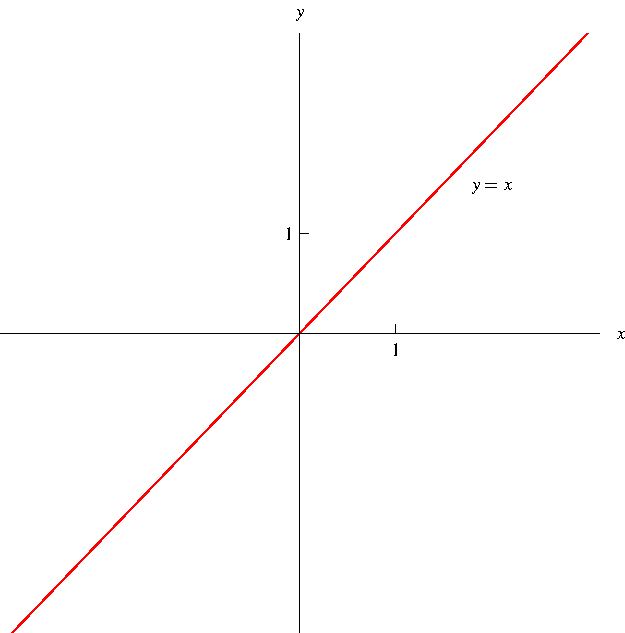
\includegraphics[height=4cm]{precalculus/pictures/01-02-x.pdf}%
%}%
%\only<handout:3| 3>{%
%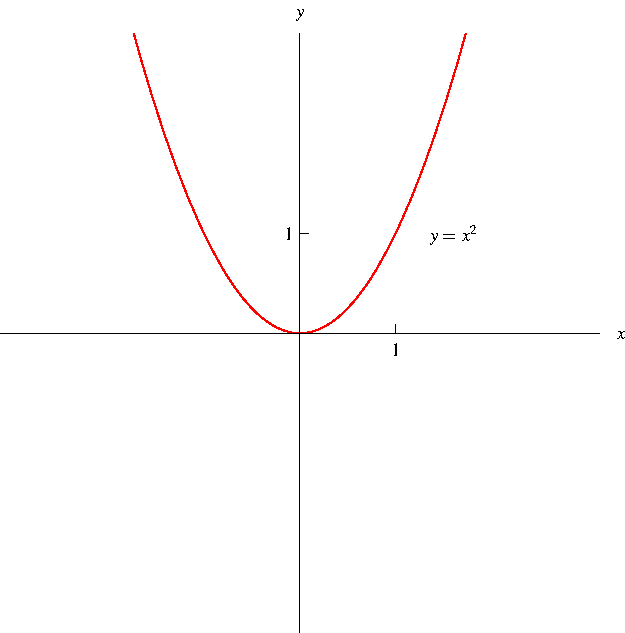
\includegraphics[height=4cm]{precalculus/pictures/01-02-xsquared.pdf}%
%}%
%\only<handout:4| 4>{%
%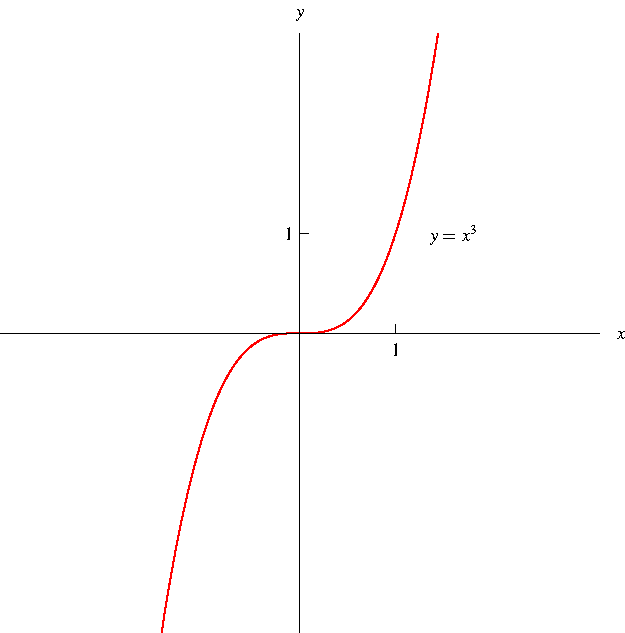
\includegraphics[height=4cm]{precalculus/pictures/01-02-xcubed.pdf}%
%}%
%\only<handout:5| 5>{%
%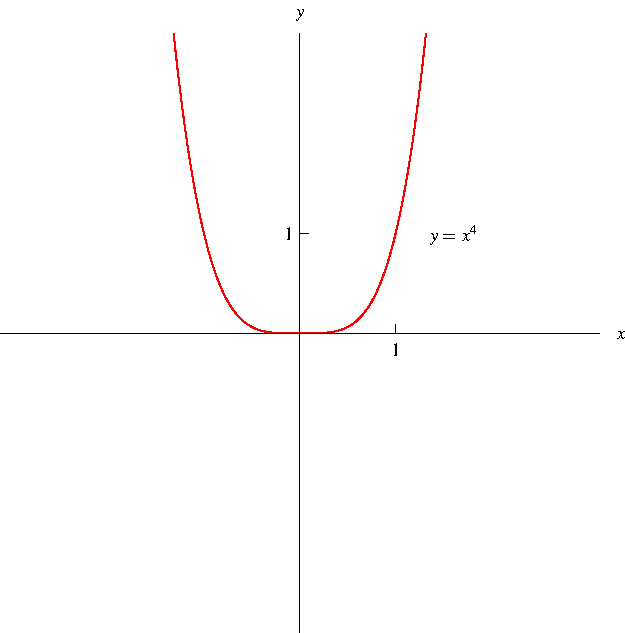
\includegraphics[height=4cm]{precalculus/pictures/01-02-xfourth.pdf}%
%}%
%\only<handout:6| 6>{%
%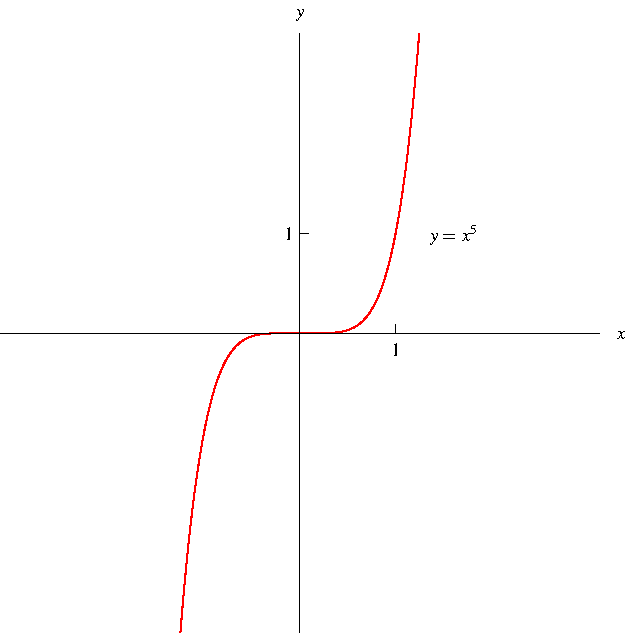
\includegraphics[height=4cm]{precalculus/pictures/01-02-xfifth.pdf}
%}%
}
\end{frame}
% end module power-functions-def

% begin module even-power-functions
\begin{frame}
\begin{tabular}{cc}
\ \only<handout:0| -2>{%
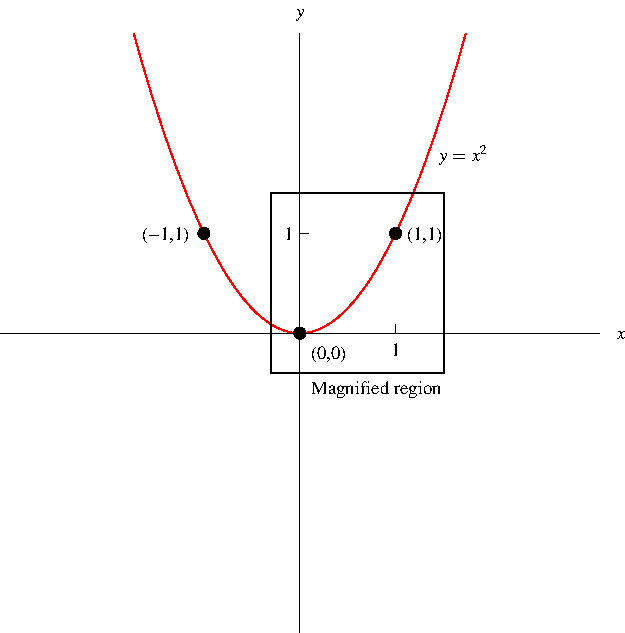
\includegraphics[height=5cm]{precalculus/pictures/01-02-evenpowersa.pdf}%
}%
\only<handout:0| 3>{%
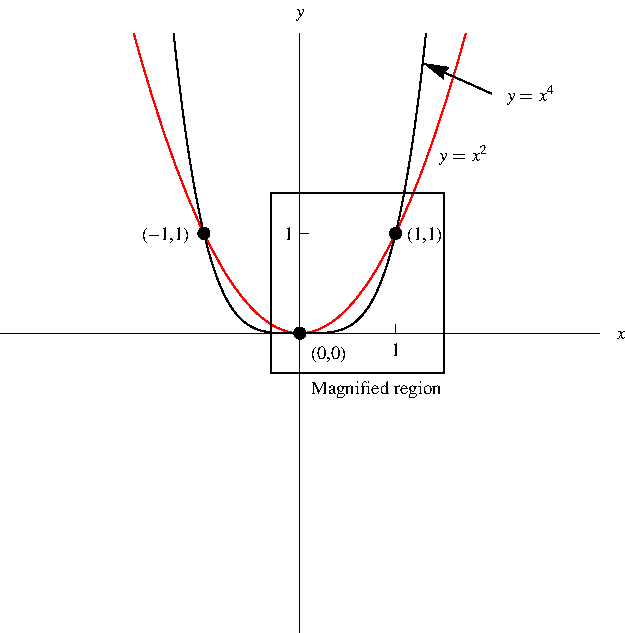
\includegraphics[height=5cm]{precalculus/pictures/01-02-evenpowersb.pdf}%
}%
\only<4>{%
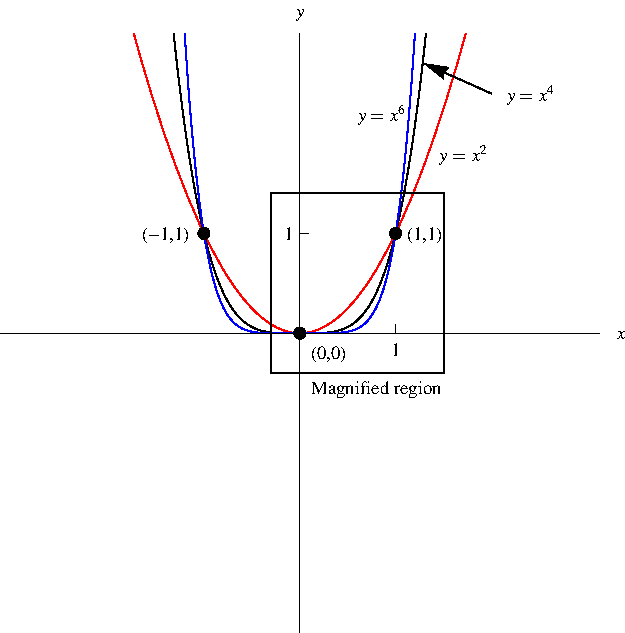
\includegraphics[height=5cm]{precalculus/pictures/01-02-evenpowersc.pdf}%
}%
&%
\ \only<handout:0| -2>{%
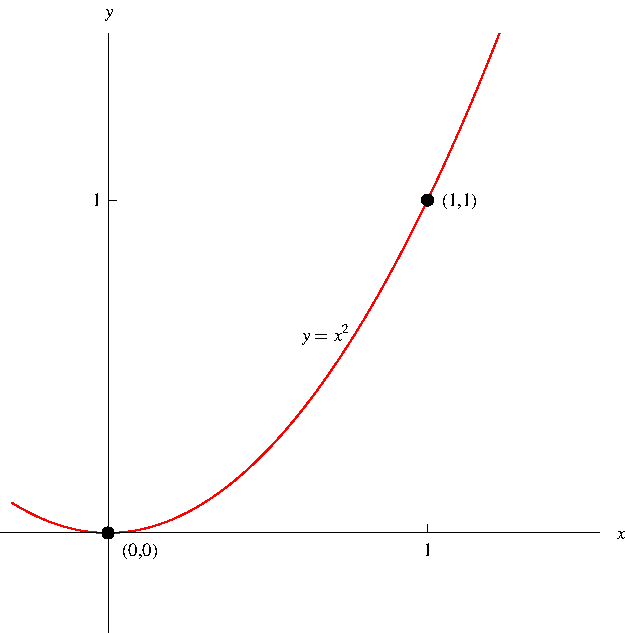
\includegraphics[height=5cm]{precalculus/pictures/01-02-evenpowerszooma.pdf}%
}%
\only<handout:0| 3>{%
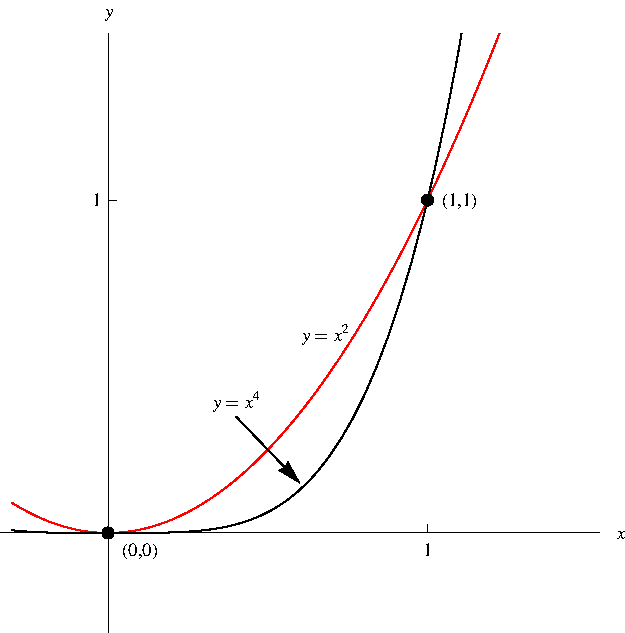
\includegraphics[height=5cm]{precalculus/pictures/01-02-evenpowerszoomb.pdf}%
}%
\only<4>{%
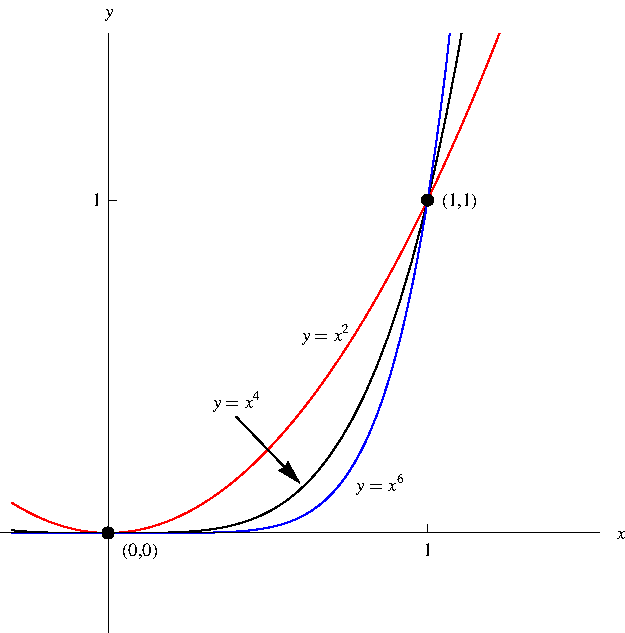
\includegraphics[height=5cm]{precalculus/pictures/01-02-evenpowerszoomc.pdf}%
}%
\end{tabular}
\begin{itemize}
\item<2->  All positive, even powers of $x$ (e.g., $x^2, x^4, \ldots$) pass through $(0,0), (-1, 1)$, and $(1,1)$.
\item<3->  If $n > m$, then $y = x^n$ is higher than $y = x^m$ when $x > 1$ or when $x < -1$, but lower when $-1 < x < 1$.
\end{itemize}
\end{frame}
% end module even-power-functions

% begin module odd-power-functions
\begin{frame}
\begin{tabular}{cc}
\ \only<handout:0| -2>{%
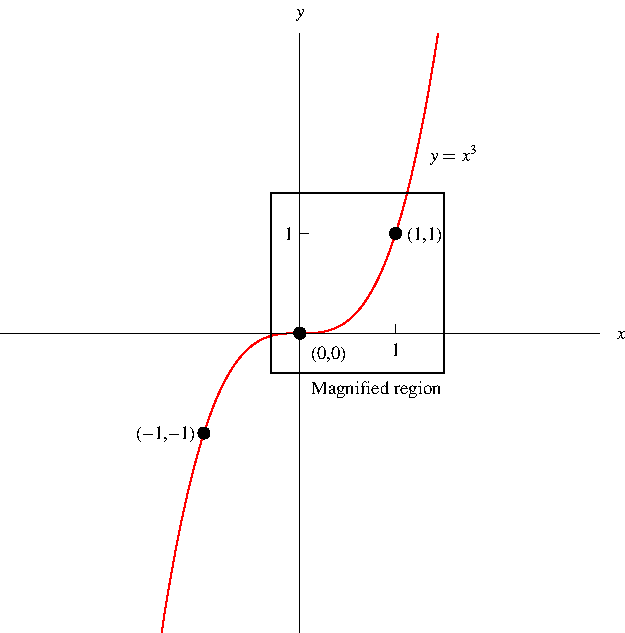
\includegraphics[height=5cm]{precalculus/pictures/01-02-oddpowersa.pdf}%
}%
\only<handout:0| 3>{%
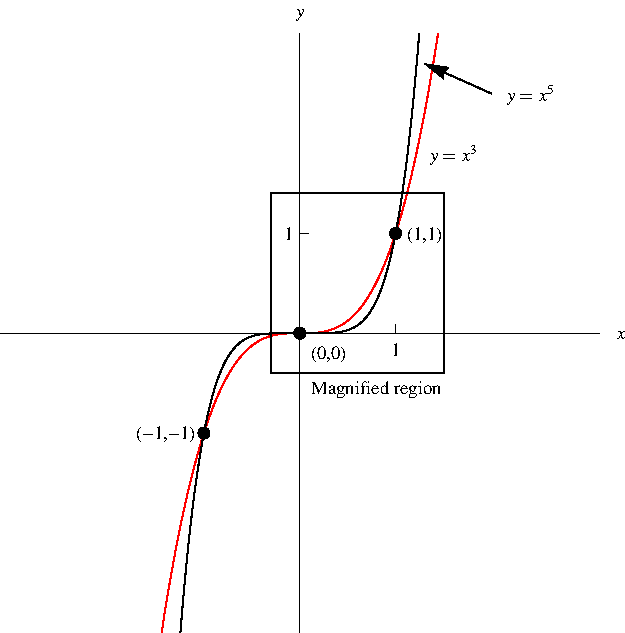
\includegraphics[height=5cm]{precalculus/pictures/01-02-oddpowersb.pdf}%
}%
\only<4>{%
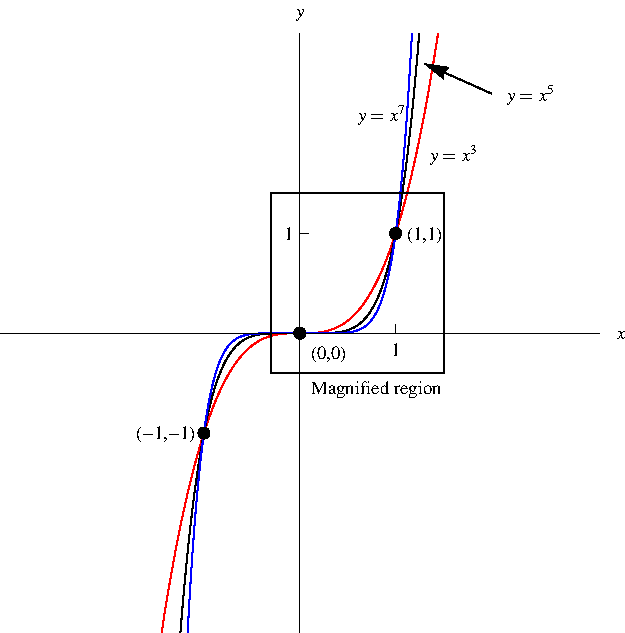
\includegraphics[height=5cm]{precalculus/pictures/01-02-oddpowersc.pdf}%
}%
&%
\ \only<handout:0| -2>{%
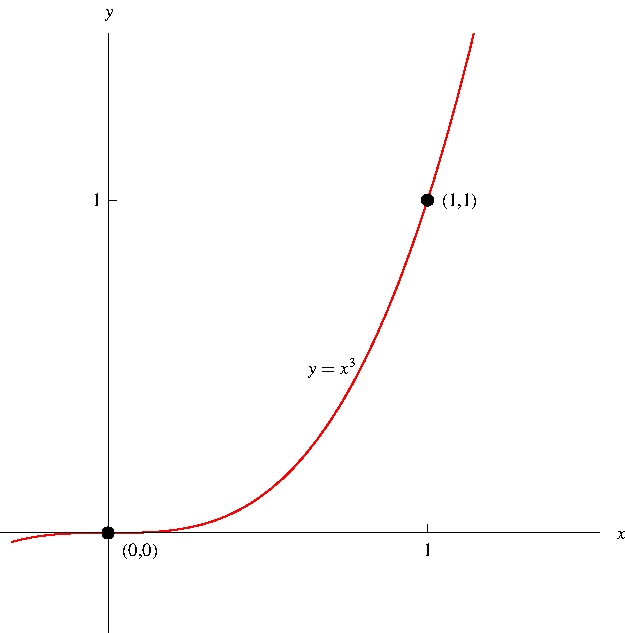
\includegraphics[height=5cm]{precalculus/pictures/01-02-oddpowerszooma.pdf}%
}%
\only<handout:0| 3>{%
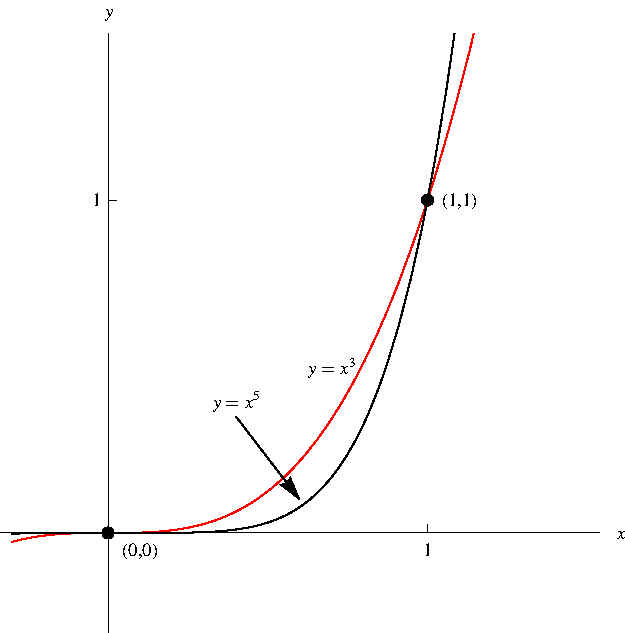
\includegraphics[height=5cm]{precalculus/pictures/01-02-oddpowerszoomb.pdf}%
}%
\only<4>{%
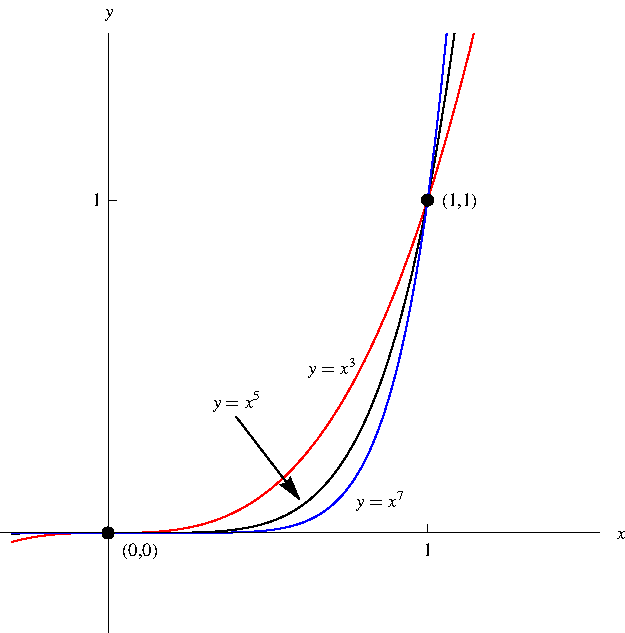
\includegraphics[height=5cm]{precalculus/pictures/01-02-oddpowerszoomc.pdf}%
}%
\end{tabular}
\begin{itemize}
\item<2->  All positive, odd powers of $x$ (e.g., $x^3, x^5, \ldots$) pass through $(0,0), (-1, -1)$, and $(1,1)$.
\item<3->  If $n > m$, then $y = x^n$ is higher than $y = x^m$ when $x > 1$ or when $-1 < x < 0$, but lower when $x < -1$ or $0 < x < 1$.
\end{itemize}
\end{frame}
% end module odd-power-functions

% begin module root-functions
\begin{frame}
\begin{itemize}
\item<1->  If $n$ is a positive integer, the function $f(x) = x^{\frac{1}{n}} = \sqrt[n]{x}$ is called a root function.
\item<2->  When $n = 2$, it is the square root function $f(x) = \sqrt{x}$.
\item<3->  The square root is not defined for negative numbers, so its domain is $[0, \infty)$.
\item<4->  Its graph is the top half of the parabola $x = y^2$.
\item<5->  The graph of the cube root function $f(x) = \sqrt[3]{x}$ is similar to that of the square root, but it is defined everywhere.
\end{itemize}
\begin{tabular}{cc}
\uncover<2->{%
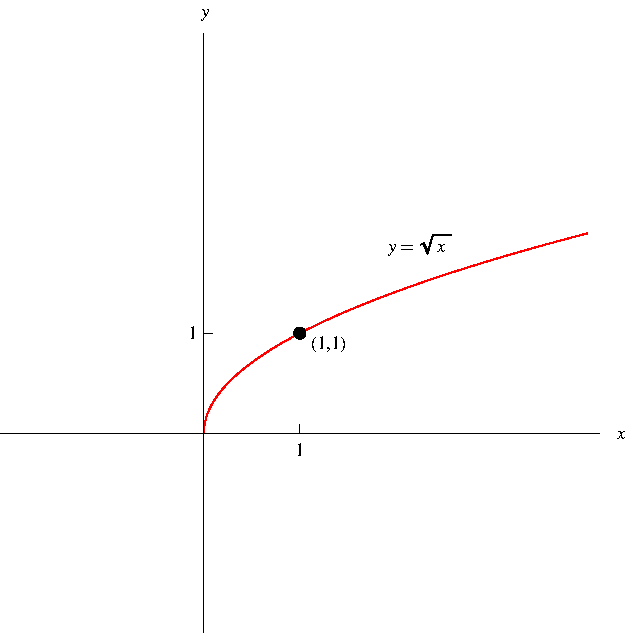
\includegraphics[height=3.5cm]{precalculus/pictures/01-02-sqrtx.pdf}%
}%
&%
\uncover<5->{%
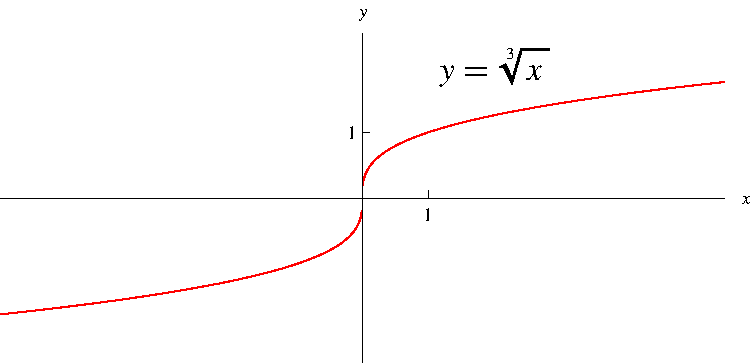
\includegraphics[height=3.5cm]{precalculus/pictures/cube-root.pdf}%
}%
\end{tabular}
\end{frame}
% end module root-functions

% begin module reciprocal-function
\begin{frame}
$f(x) = x^{-1} = \frac{1}{x}$ is called the reciprocal function.  Its graph has equation $y = \frac{1}{x}$, or $xy = 1$, and is an hyperbola with the coordinate axes as its asymptotes.
%\begin{center}%center does not work with well with pstricks and pgflayout.
\hfil\hfil\psset{xunit=0.6cm, yunit=0.6cm}
\begin{pspicture}(-5, -5)(5,5)
\psframe*[linecolor=white](-5,-5)(5,5)
\psaxes[ticks=none, labels=none]{<->}(0,0)(-5,-5)(5,5)\tiny
%Function formula: (1)/(x)
\rput(1,3){$y=\frac 1 x$}
\psplot[linecolor=red, plotpoints=1000]{0.2}{5}{1 x div } %Function formula: (1)/(x)
\rput(1,3){$y=\frac 1 x$}
\psplot[linecolor=red, plotpoints=1000]{-5}{-0.2}{1 x div }
\fcLabels{4.5}{4.5}
\end{pspicture}
%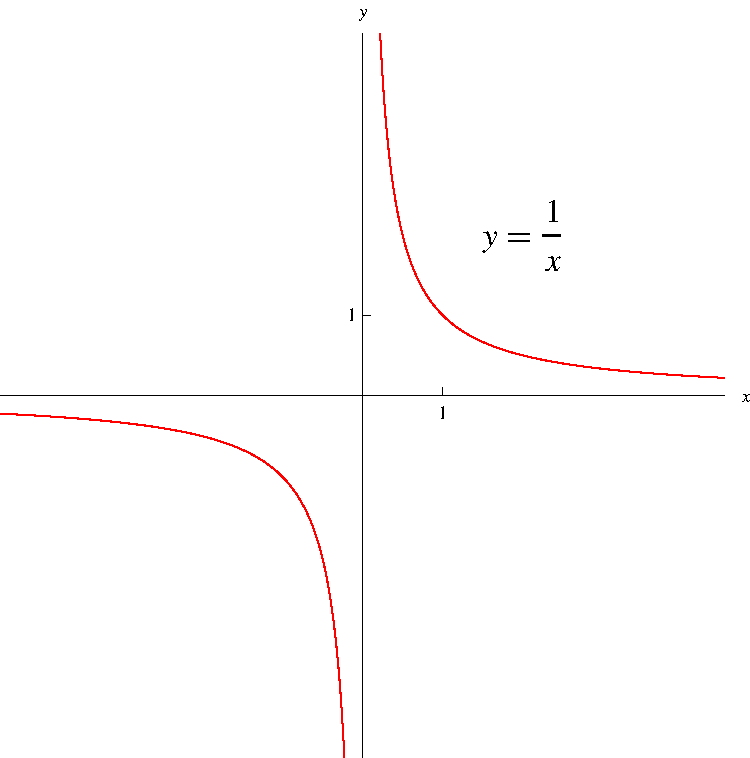
\includegraphics[height=5cm]{precalculus/pictures/reciprocal-function.pdf}%
%\end{center}
\end{frame}
% end module reciprocal-function

\subsection{Rational Functions}
% begin module rational-functions
\begin{frame}
\frametitle{Rational Functions}
\begin{definition}[Rational Function]
A rational function is a quotient of two polynomials; that is, a function of the form
\[
f(x) = \frac{g(x)}{h(x)},
\]
where $g$ and $h$ are polynomials.
\end{definition}
\begin{columns}[c]
\column{.4\textwidth}
\uncover<2->{
\psset{xunit=0.4cm, yunit=0.4cm}
\begin{pspicture}(-5, -5)(5,5) 
\psframe*[linecolor=white](-5,-5)(5,5) 
\psaxes[ticks=none, labels=none]{<->}(0,0)(-4.5,-4.5)(4.5,4.5)\tiny
%Function formula: \frac{x}{(x)^{2}-1} 
\rput(2.5,-3){$y=\frac{x}{x^{2}-1}$} 
\psplot[linecolor=red, plotpoints=1000]{1.11727}{4.5}{x -1 x 2 exp add div } %Function formula: \frac{x}{(x)^{2}-1} 
\psplot[linecolor=red, plotpoints=1000]{-0.895043}{0.895043}{x -1 x 2 exp add div } %Function formula: \frac{x}{(x)^{2}-1} 
\psplot[linecolor=red, plotpoints=1000]{-4.5}{-1.11727}{x -1 x 2 exp add div }
\psLabels{4.5}{4.5}
\end{pspicture} 
%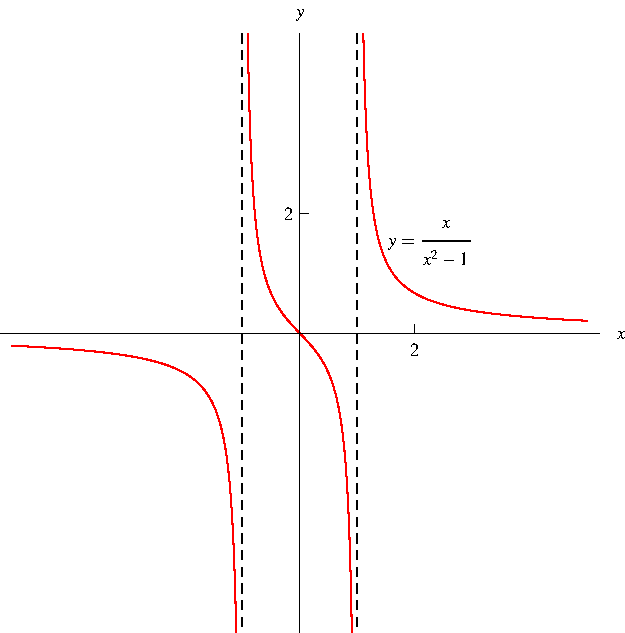
\includegraphics[height=4cm]{precalculus/pictures/01-02-rational.pdf}%
}
\column{.6\textwidth}
\uncover<2->{
\begin{example}[$x/(x^2-1)$]
The function
\[
f(x) = \frac{x}{x^2-1}
\]
is a rational function.
\end{example}
}
\end{columns}
\end{frame}
% end module rational-functions

\subsection{Algebraic Functions}
%Old Version from Greg. Greg, this slide is changed substantially, please take a look.
%% begin module algebraic-functions
%\begin{frame}
%\frametitle{Algebraic Functions}
%\begin{definition}[Algebraic Function]
%An algebraic function is a function that can be constructed using algebraic operations (such as addition, subtraction, multiplication, division, and taking roots) starting from polynomials.
%\end{definition}
%\uncover<2->{
%Algebraic functions can look pretty funny.
%\begin{tabular}{ccc}
%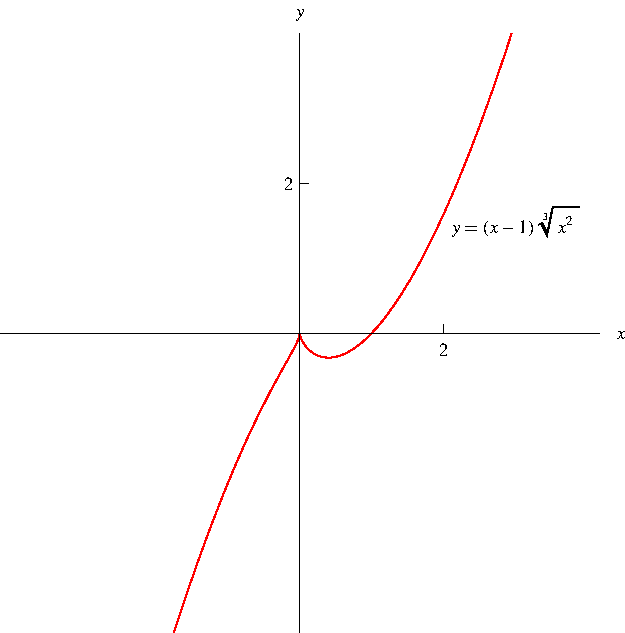
\includegraphics[height=3.8cm]{precalculus/pictures/01-02-algebraic1.pdf}&%
%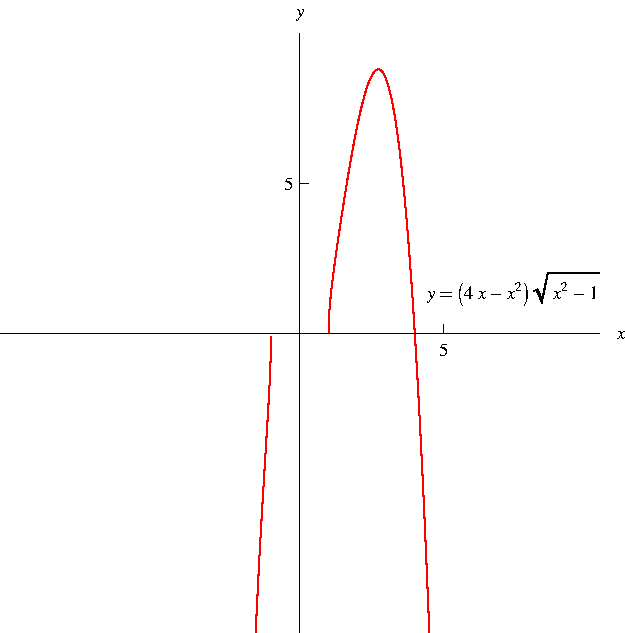
\includegraphics[height=3.8cm]{precalculus/pictures/01-02-algebraic2.pdf}&%
%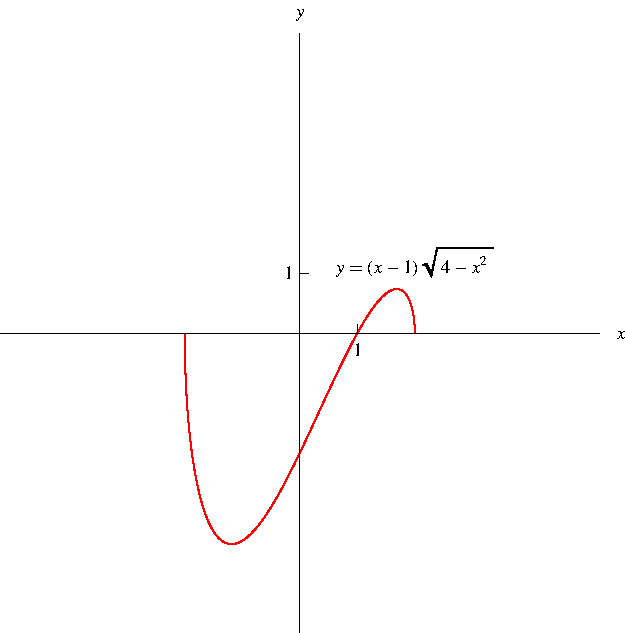
\includegraphics[height=3.8cm]{precalculus/pictures/01-02-algebraic3.pdf}%
%\end{tabular}
%}
%\end{frame}
%% end module algebraic-functions


% begin module algebraic-functions
\begin{frame}
\frametitle{Algebraic Functions}
\begin{definition}[Algebraic Function]
A function in $x$ that can be constructed using $x$, constants, and finitely many of the operations $+, -, *, /,$ and $\sqrt[n]{~}$ is an algebraic function.

\uncover<2->{{\footnotesize Outside of Calculus I: function $f(x)$ = algebraic if it satisfies a polynomial equation with polynomial coefficients, i.e., $a_0(x) +a_1(x)f(x)+\dots +a_n(x) \left(f(x)\right)^n=0$ for some polynomials  $a_i(x)$.}}
\end{definition}
\uncover<3->{
Examples.

\begin{tabular}{ccc}
\psset{xunit=0.3cm, yunit=0.3cm}
\begin{pspicture}(-5, -5)(5,5)
\tiny\psframe*[linecolor=white](-5,-5)(5,5)
\psaxes[ticks=none, labels=none]{<->}(0,0)(-4.5,-4.5)(4.5,4.5)\tiny
%Function formula: - ((- (x))^{5/3})- ((- (x))^{2/3})
\psplot[linecolor=red, plotpoints=1000]{-2}{-0.001}{x -1 mul 0.666667 exp -1 mul x -1 mul 1.66667 exp -1 mul add } %Function formula: (x)^{5/3}- ((x)^{2/3})
\rput[t](1,-5){$y=(x-1)\sqrt[3]{x^2}$}
\psplot[linecolor=red, plotpoints=1000]{0.001}{3}{x 0.666667 exp -1 mul x 1.66667 exp add }
\fcLabels{4.5}{4.5}
\end{pspicture}
%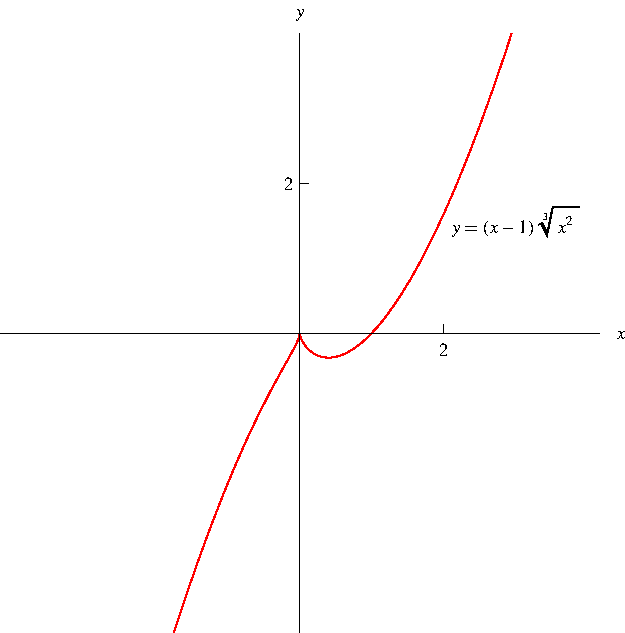
\includegraphics[height=3.8cm]{precalculus/pictures/01-02-algebraic1.pdf}
&%
\psset{xunit=0.3cm, yunit=0.3cm}
\begin{pspicture}(-5, -5)(5,5)
\tiny\psframe*[linecolor=white](-5,-5)(5,5)
\psaxes[ticks=none, labels=none]{<->}(0,0)(-4.5,-4.5)(4.5,4.5)\tiny
\psplot[linecolor=red, plotpoints=1000]{1}{5}{-1 x 2 exp add 0.5 exp x 2 exp mul -0.2 mul -1 x 2 exp add 0.5 exp x mul 0.8 mul add } %Function formula: 4/5 ((x) (((x)^{2}-1)^{1/2}))-1/5 (((x)^{2}) (((x)^{2}-1)^{1/2}))
\rput[t](1,-5){$y=\frac15(4x-x^2)\sqrt{x^2-1}$}
\psplot[linecolor=red, plotpoints=1000]{-2}{-1}{-1 x 2 exp add 0.5 exp x 2 exp mul -0.2 mul -1 x 2 exp add 0.5 exp x mul 0.8 mul add }
\fcLabels{4.5}{4.5}
\end{pspicture}
%\includegraphics[height=3.8cm]{precalculus/pictures/01-02-algebraic2.pdf}
&%
\psset{xunit=0.3cm, yunit=0.3cm}
\begin{pspicture}(-5, -5)(5,5)
\tiny\psframe*[linecolor=white](-5,-5)(5,5)
\psaxes[ticks=none, labels=none]{<->}(0,0)(-4.5,-4.5)(4.5,4.5)\tiny
%Function formula: - ((4- ((x)^{2}))^{1/2})+(x) ((4- ((x)^{2}))^{1/2})
\rput[t](1,-5){$y=(x-1)\sqrt{4-x^2}$}
\psplot[linecolor=red, plotpoints=1000]{-2}{2}{x 2 exp -1 mul 4 add 0.5 exp x mul x 2 exp -1 mul 4 add 0.5 exp -1 mul add }
\fcLabels{4.5}{4.5}
\end{pspicture}
%\includegraphics[height=3.8cm]{precalculus/pictures/01-02-algebraic3.pdf}
%
\end{tabular}
}
\end{frame}
% end module algebraic-functions

% end lecture
\end{document}
